\section{Construcción}

\subsection{Módulo de carga y alimentación}

Dentro del sistema es crítico el constante monitoreo de las variables de orientación,
temperatura y respiración del bebé, para ello se utilizó una batería \acrshort{li-po} para mantener
alimentado el sistema. Al no poderse utilizar únicamente la batería de forma directa, se
diseño el siguiente módulo de carga y alimentación, el cual esta construido por 3 partes:

\begin{figure}[htp!]
    \centering
    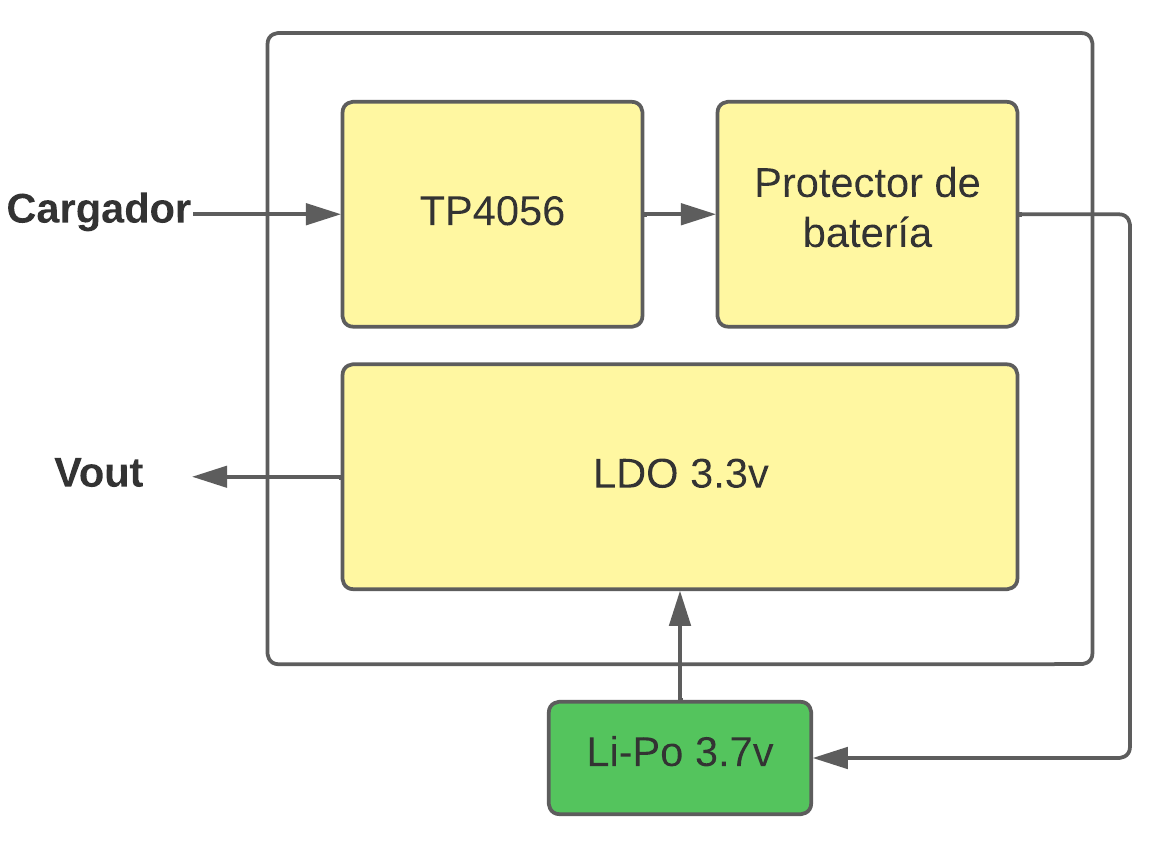
\includegraphics[width=\columnwidth]{charging_and_power_supply_module.png}
    \caption{Partes que conforman el módulo de carga y alimentación.}
    \label{fig: charging_and_power_module}
\end{figure}
\FloatBarrier

\begin{figure}[htp!]
    \centering
    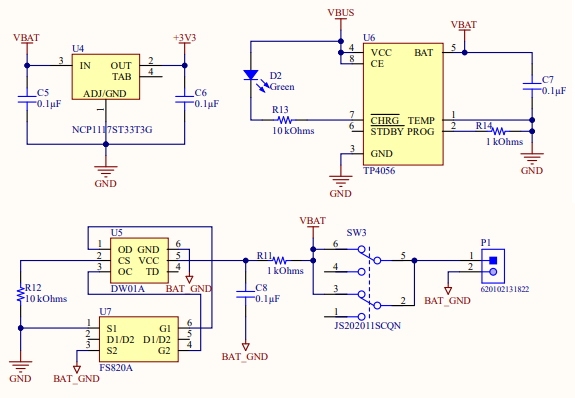
\includegraphics[width=\columnwidth]{battery_module_schematic.png}
    \caption{Esquemáticos del módulo de carga y alimentación.}
    \label{fig: battery_module_schematic}
\end{figure}
\FloatBarrier

\subsection{Diseño de \acrshort{pcb}}

\subsubsection{Layout}
El diseño del \acrshort{pcb} se realizo siguiendo una visión de obtener un dispositivo
mínimo y pequeño para evitar incomodidades en el bebé.

A continuación se muestra el layout final de la primera versión:

\begin{figure}[htp!]
    \centering
    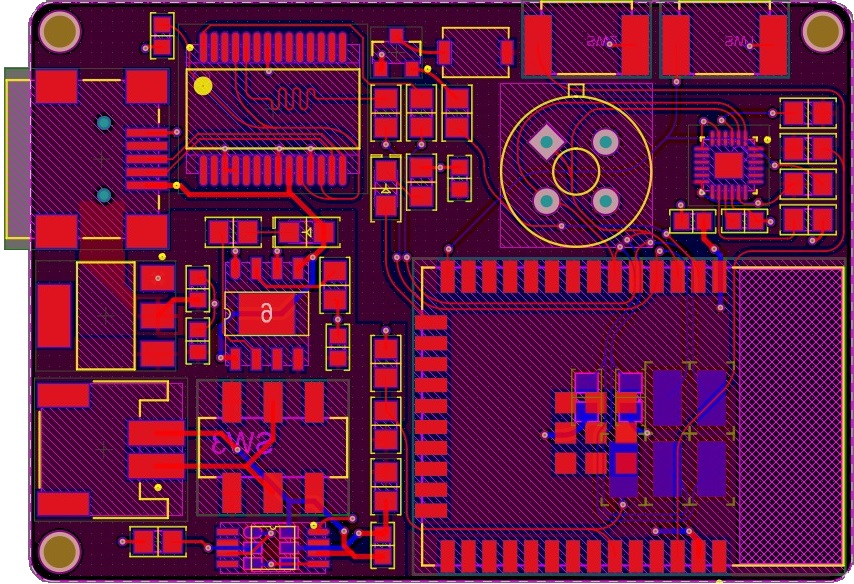
\includegraphics[width = 0.38 \textwidth]{layout.jpeg}
    \caption{Layout del \acrshort{pcb}.}
    \label{fig: layout}
\end{figure}
\FloatBarrier

\subsubsection{PCB 3D}
\begin{figure}[htp!]
    \centering
    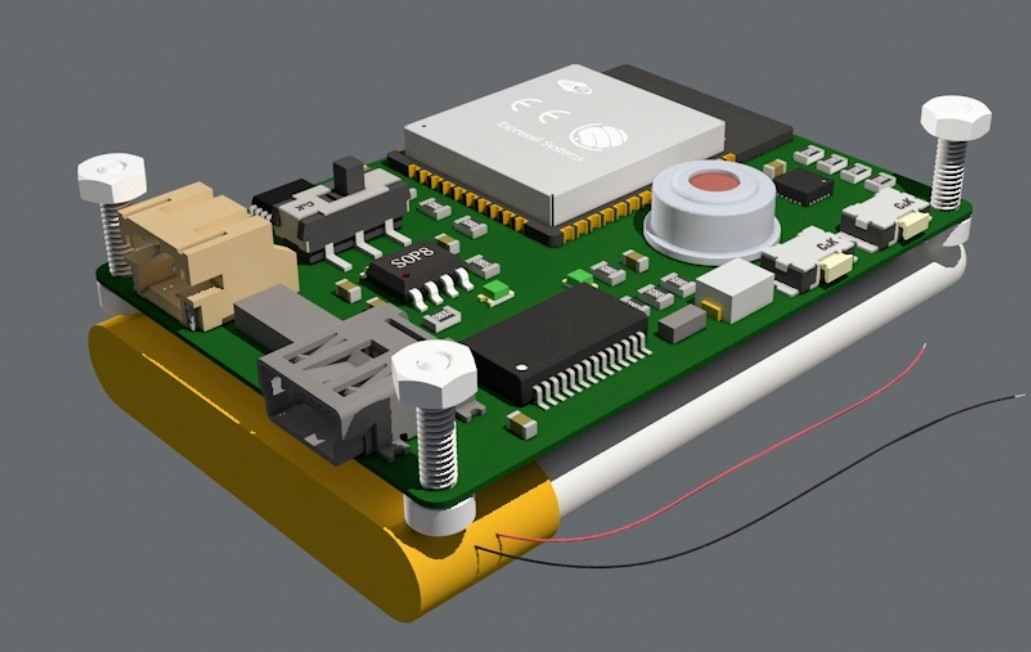
\includegraphics[width = 0.38 \textwidth]{isometric_view_3D.jpg}
    \caption{Vista isométrica del \acrshort{pcb} y la batería.}
    \label{fig: isometric_3d}
\end{figure}
\FloatBarrier

En las figuras \ref{fig: isometric_3d} y \ref{fig: top_3d} se muestra el modelo 3D, este fue hecho
para poder corraborar de que tamaño quedaría el dispositivo final contando la \acrshort{pcb} y la batería.

Tanto el modelo 3D como el layout de la \acrshort{pcb} fue diseñado en el software Altium.
\subsection{Diseño de Carcasa}
\begin{figure}[htp!]
    \centering
    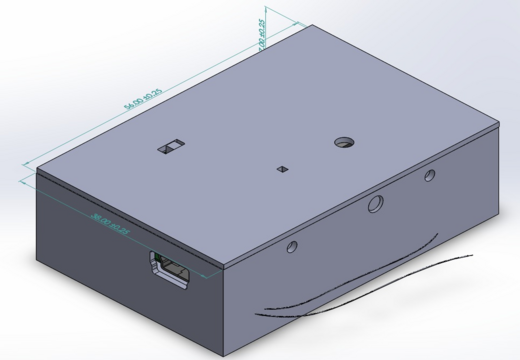
\includegraphics[width=\columnwidth]{system_shell_v2.png}
    \caption{Vista isométrica de la carcasa}
    \label{fig: isometric_view_shell}
\end{figure}
\FloatBarrier

\begin{figure}[htp!]
    \centering
    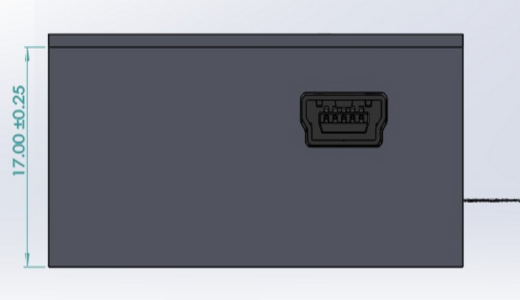
\includegraphics[width=\columnwidth]{front_view_system_shell_v2.png}
    \caption{Vista de la parte frontal de la carcasa, donde esta el puerto USB}
    \label{fig: front_view_shell}
\end{figure}
\FloatBarrier

\begin{figure}[htp!]
    \centering
    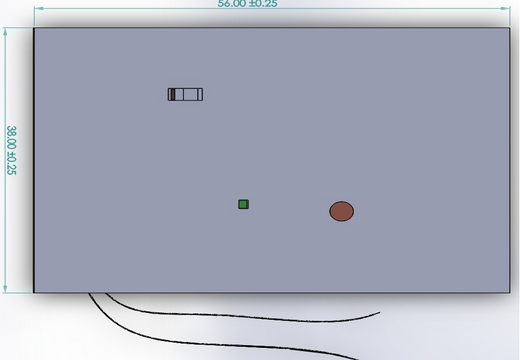
\includegraphics[width=\columnwidth]{top_view_syste_shell_v2.png}
    \caption{Vista superior de la carcasa}
    \label{fig: top_view_shell}
\end{figure}
\FloatBarrier


En las figuras \ref{fig: front_view_shell} y \ref{fig: top_view_shell}, 
se puede ver el diseño propuesto para la carcasa del sistema, donde esta 
tendrá las siguientes aberturas:

\begin{itemize}
    \item Switch encendido/apagado
    \item Puerto de carga Micro-USB tipo-B
    \item Salida para el sonido del buzzer
    \item Led infrarrojo del sensor de temperatura
\end{itemize}

